\makeatletter
\let\inserttitle\@title
\makeatother

\makeatletter
\let\insertauthor\@author
\makeatother

\makeatletter
\let\insertdate\@date
\makeatother

\newgeometry{left=1.8cm,bottom=0cm,right=1.8cm}

\begin{center}

\vspace*{-4cm}

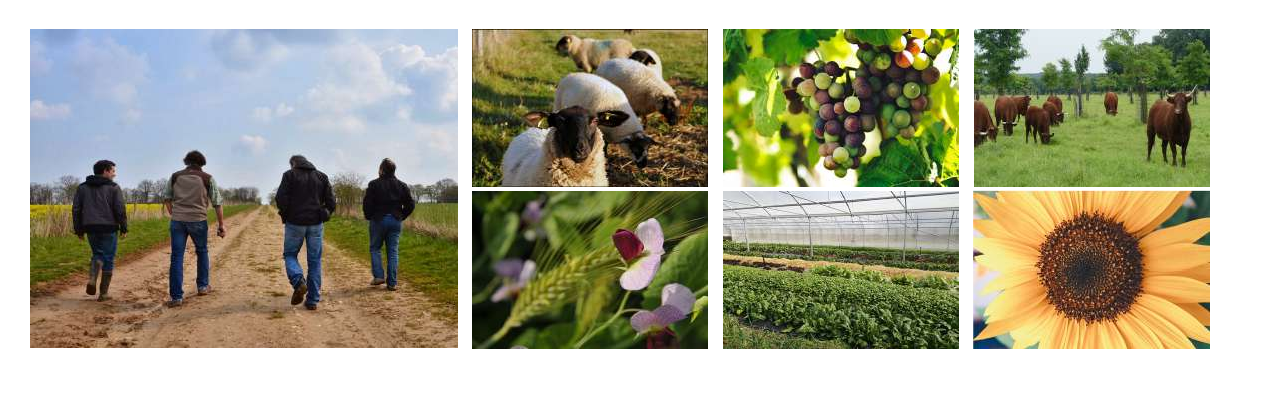
\includegraphics[width=\textwidth]{templates/banner_group.pdf}

\vspace*{1cm}

{\sffamily\huge\bfseries \textbf{\inserttitle}}\par\bigskip


\includegraphics[]{templates/IDEA_Horizontal}

\end{center}

\begin{flushright}

\hspace{-1cm}{\Large \sffamily Analyse de durabilité des exploitations agricoles : \par \textbf{\insertauthor}}\par

\vspace*{1cm}

\end{flushright}

\begin{center}
\begin{onehalfspace}

\hspace{-1cm}{\large \sffamily \color{red} \textbf{NB : Analyse reposant sur un échantillon d'une base de données non représentative des exploitations agricoles françaises}}\par
\end{onehalfspace}
\end{center}

\vspace*{-0.6cm}

Document type de restitution des résultats issu des travaux de :
\vspace*{-0.5cm}
\begin{figure}

\includegraphics[height=1.5cm]{templates/casdar} \hspace{0.2cm}

\includegraphics[height=1.5cm]{templates/logotype-INRAE-ETTIS} \hspace{0.3cm}
\vspace*{0.5cm}
\includegraphics[height=2.5cm]{templates/bergerie}\hspace{-0.5cm}

\includegraphics[height=2.2cm]{templates/logo_bsa_Vertical_cmjn}\par
\end{figure}

\vspace*{-2cm}

\begin{center}
\makebox[0pt][l]{%
\hspace{-11.4cm}
\raisebox{-\totalheight}[0pt][0pt]{%

\includegraphics[width=230mm]{templates/foot_green.png}}}%
\end{center}

\restoregeometry

